% sec3_results.tex — 第3节 结果
\section{结果}

\subsection{实验设置}

为验证第~\ref{subsec:modification}~节所述改动的有效性，设计了以下实验组别：

\begin{table}[H]
\centering
\caption{实验组别设置}
\label{tab:exp-groups}
\begin{tabular}{llll}
\toprule
\textbf{组别}     & \textbf{标识}    & \textbf{核心差异}              & \textbf{说明} \\
\midrule
基线               & Baseline         & 原始 SuGaR 提取流程            & 无剔点 \\
改动（$\tau{=}0.05$）  & Modified-0.05  & 多视角剔点\,$\tau{=}0.05$  & 剔除 25.5\% \\
改动（$\tau{=}0.02$）  & Modified-0.02  & 多视角剔点\,$\tau{=}0.02$  & 默认值，剔除 44.9\% \\
改动（$\tau{=}0.01$）  & Modified-0.01  & 多视角剔点\,$\tau{=}0.01$  & 剔除 59.2\% \\
\bottomrule
\end{tabular}
\end{table}

所有组别共享同一 3DGS 预训练检查点（7{,}000 迭代、\texttt{seed}=0）、
相同的 Coarse SuGaR 权重（\texttt{num\_iterations}=15{,}000）以及相同的
测试视角划分（\texttt{llffhold}=8，32 个测试视角）。
改动仅作用于 Mesh 提取阶段，不影响 3DGS 与 Coarse SuGaR 的训练过程。

\textbf{评价指标}包括五个维度：
\begin{itemize}[nosep]
  \item 渲染质量：测试视角 PSNR / SSIM / LPIPS（\S\ref{ssec:baseline-render}）；
  \item 几何精度：双参考 Accuracy / Completeness / Chamfer / F-score（\S\ref{ssec:baseline-geo}）；
  \item 拓扑质量：连通分量数、水密性、孔洞数等（\S\ref{ssec:baseline-topo}）；
  \item 覆盖度：网格渲染覆盖率与前景漏洞率（\S\ref{ssec:baseline-topo}）；
  \item 效率：各阶段墙钟时间、峰值显存与文件体积（\S\ref{ssec:baseline-topo}）。
\end{itemize}

% =====================================================================
\subsection{定量结果}
\label{ssec:baseline-results}

以下报告全部实验组别在 truck 场景上的定量结果。

% ---------- 渲染指标 ----------
\subsubsection{渲染指标}
\label{ssec:baseline-render}

表~\ref{tab:render-metrics} 给出 3DGS（7k 迭代）与 Coarse SuGaR 在 32 个测试视角
上的渲染质量。由于改动仅影响 Mesh 提取阶段，不改变 3DGS 或 Coarse SuGaR
的训练权重，因此所有组别共享同一 Coarse 模型，渲染指标恒等。

\begin{table}[H]
\centering
\caption{渲染指标（truck，32 测试视角均值）。
各组别共享同一 Coarse SuGaR 模型，故渲染指标与基线恒等。}
\label{tab:render-metrics}
\begin{tabular}{lccc}
\toprule
\textbf{模型} & \textbf{PSNR (dB) $\uparrow$}
               & \textbf{SSIM $\uparrow$}
               & \textbf{LPIPS $\downarrow$} \\
\midrule
3DGS（7k 迭代）   & 23.92 & 0.849 & 0.202 \\
Coarse SuGaR       & 24.32 & 0.848 & 0.217 \\
\bottomrule
\end{tabular}
\end{table}

% ---------- 几何指标 ----------
\subsubsection{几何指标}
\label{ssec:baseline-geo}

表~\ref{tab:geo-refA} 与表~\ref{tab:geo-refB} 分别给出以 3DGS 高斯中心（参考 A）
和 COLMAP 稀疏点云（参考 B）为基准的几何评测结果。
所有距离均以场景坐标为单位（场景对角线~$\approx$\,13.34）。
$\tau$ 越小，剔点越激进，几何精度（Chamfer / Completeness / F-score）一致改善，
但精度尾部（Accuracy P90）逐渐变差，反映了真实表面被误剔的趋势。

\begin{table}[H]
\centering\small
\caption{几何指标——参考 A（3DGS 高斯中心，284{,}309 点）}
\label{tab:geo-refA}
\begin{tabular}{@{}lcccc@{}}
\toprule
\textbf{指标} & \textbf{基线} & $\tau{=}0.05$ & $\tau{=}0.02$ & $\tau{=}0.01$ \\
\midrule
Chamfer L1 $\downarrow$          & 0.0326 & 0.0287 & 0.0242 & 0.0230 \\
\addlinespace
Accuracy 均值 $\downarrow$       & 0.0156 & 0.0184 & 0.0198 & 0.0220 \\
Accuracy 中位 $\downarrow$       & 0.0098 & 0.0103 & 0.0105 & 0.0110 \\
Accuracy P90 $\downarrow$        & 0.0291 & 0.0327 & 0.0343 & 0.0366 \\
\addlinespace
Completeness 均值 $\downarrow$   & 0.0495 & 0.0389 & 0.0286 & 0.0241 \\
Completeness 中位 $\downarrow$   & 0.0233 & 0.0183 & 0.0148 & 0.0138 \\
Completeness P90 $\downarrow$    & 0.1317 & 0.0995 & 0.0593 & 0.0490 \\
\addlinespace
F@0.5\% $\uparrow$              & 0.864 & 0.902 & 0.940 & 0.952 \\
F@1\% $\uparrow$                & 0.946 & 0.961 & 0.976 & 0.982 \\
F@2\% $\uparrow$                & 0.990 & 0.993 & 0.994 & 0.995 \\
\bottomrule
\end{tabular}
\end{table}

\begin{table}[H]
\centering\small
\caption{几何指标——参考 B（COLMAP 稀疏点，56{,}988 点）}
\label{tab:geo-refB}
\begin{tabular}{@{}lcccc@{}}
\toprule
\textbf{指标} & \textbf{基线} & $\tau{=}0.05$ & $\tau{=}0.02$ & $\tau{=}0.01$ \\
\midrule
Chamfer L1 $\downarrow$          & 0.0531 & 0.0455 & 0.0390 & 0.0361 \\
\addlinespace
Accuracy 均值 $\downarrow$       & 0.0242 & 0.0262 & 0.0279 & 0.0303 \\
Accuracy 中位 $\downarrow$       & 0.0033 & 0.0035 & 0.0036 & 0.0037 \\
Accuracy P90 $\downarrow$        & 0.0200 & 0.0239 & 0.0258 & 0.0287 \\
\addlinespace
Completeness 均值 $\downarrow$   & 0.0819 & 0.0648 & 0.0500 & 0.0419 \\
Completeness 中位 $\downarrow$   & 0.0480 & 0.0387 & 0.0307 & 0.0271 \\
Completeness P90 $\downarrow$    & 0.2005 & 0.1530 & 0.1044 & 0.0853 \\
\addlinespace
F@0.5\% $\uparrow$              & 0.751 & 0.807 & 0.862 & 0.885 \\
F@1\% $\uparrow$                & 0.888 & 0.920 & 0.949 & 0.963 \\
F@2\% $\uparrow$                & 0.963 & 0.973 & 0.979 & 0.982 \\
\bottomrule
\end{tabular}
\end{table}

% ---------- 拓扑 / 覆盖 / 效率 ----------
\subsubsection{拓扑、覆盖与效率}
\label{ssec:baseline-topo}

表~\ref{tab:topo-cov-eff} 汇总了网格拓扑质量、渲染覆盖度与效率指标。

\begin{table}[H]
\centering\footnotesize
\caption{拓扑、覆盖与效率指标（truck 场景）}
\label{tab:topo-cov-eff}
\begin{tabular}{llcccc}
\toprule
\textbf{类别} & \textbf{指标}
  & \textbf{基线} & $\tau{=}0.05$ & $\tau{=}0.02$ & $\tau{=}0.01$ \\
\midrule
\multirow{7}{*}{拓扑}
  & 顶点数 $V$           & 746{,}704
                                      & 665{,}745 & 574{,}239 & 455{,}839 \\
  & 面数 $F$             & 1{,}437{,}272
                                      & 1{,}295{,}321 & 1{,}121{,}525 & 890{,}054 \\
  & 连通分量数           & 4{,}851   & 3{,}279   & 2{,}690   & 2{,}261 \\
  & 最大分量面数占比     & 49.5\%    & 58.1\%    & 48.8\%    & 47.3\% \\
  & 边界边数             & 96{,}544  & 68{,}205  & 54{,}647  & 44{,}848 \\
  & 孔洞数（边界环）     & 7{,}970   & 6{,}206   & 5{,}480   & 4{,}598 \\
  & 水密                 & 否         & 否         & 否         & 否 \\
\midrule
\multirow{2}{*}{覆盖}
  & 网格覆盖率 $\uparrow$    & 92.9\% & 81.5\% & 71.0\% & 63.3\% \\
  & 前景漏洞率 $\downarrow$  & 6.7\%  & 18.0\% & 28.6\% & 36.3\% \\
\midrule
\multirow{6}{*}{效率}
  & 3DGS 训练            & 1.98\,min
                                      & \multicolumn{3}{c}{（共享）} \\
  & Coarse SuGaR 训练    & 15.84\,min
                                      & \multicolumn{3}{c}{（共享）} \\
  & Mesh 提取            & 5.98\,min & 4.79\,min & 4.30\,min & 3.91\,min \\
  & \textbf{总墙钟}      & \textbf{23.81\,min}
                                      & \textbf{22.62\,min}
                                      & \textbf{22.13\,min}
                                      & \textbf{21.74\,min} \\
  & 峰值显存（进程组）   & 10{,}098\,MiB
                                      & 8{,}274\,MiB & 8{,}274\,MiB & 8{,}274\,MiB \\
  & 网格文件体积         & 54.34\,MiB
                                      & 48.56\,MiB & 41.94\,MiB & 33.29\,MiB \\
\bottomrule
\end{tabular}
\begin{flushleft}
\footnotesize
"（共享）"表示该阶段在基线与改动之间相同（改动仅作用于提取阶段）。
\end{flushleft}
\end{table}

% ---------- 可视化 ----------
\subsubsection{可视化}
\label{ssec:baseline-vis}

图~\ref{fig:baseline-vis} 展示了基线提取网格的四个可视化视角。

\begin{figure}[htbp]
  \centering
  \begin{subfigure}[b]{0.48\textwidth}
    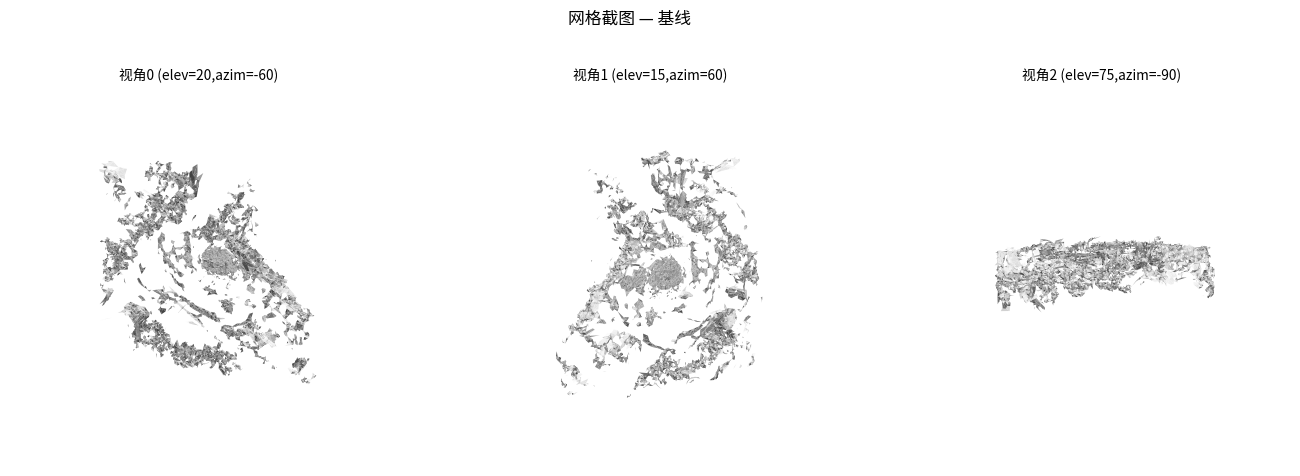
\includegraphics[width=\textwidth]{figures/网格截图_基线.png}
    \caption{提取网格整体视图}
    \label{fig:baseline-mesh}
  \end{subfigure}
  \hfill
  \begin{subfigure}[b]{0.48\textwidth}
    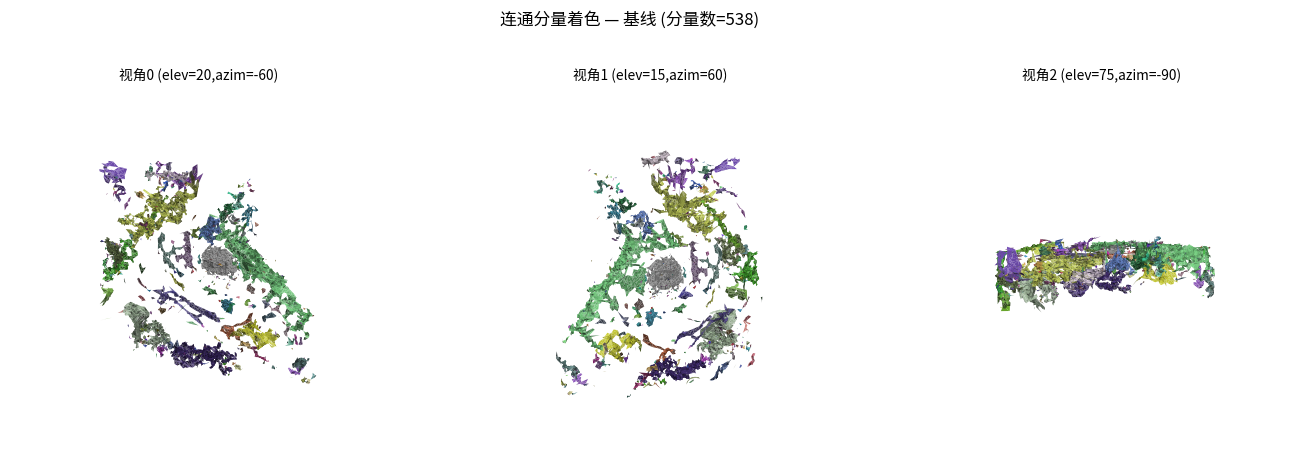
\includegraphics[width=\textwidth]{figures/连通分量着色_基线.png}
    \caption{连通分量着色（不同颜色代表不同分量）}
    \label{fig:baseline-components}
  \end{subfigure}

  \vspace{0.5em}

  \begin{subfigure}[b]{0.48\textwidth}
    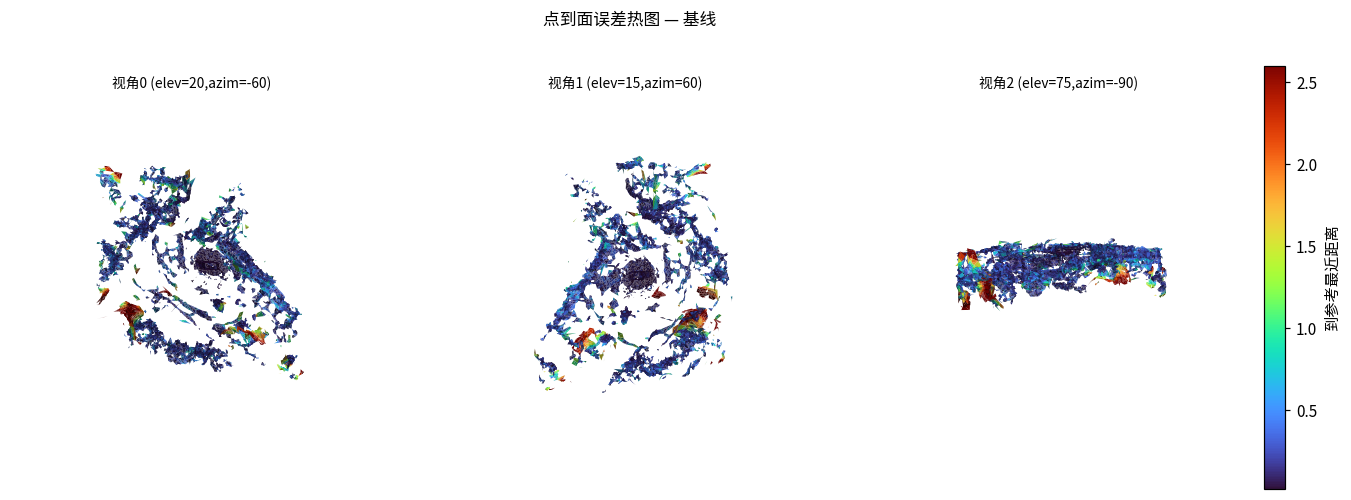
\includegraphics[width=\textwidth]{figures/误差热图_基线.png}
    \caption{几何误差热图}
    \label{fig:baseline-error}
  \end{subfigure}
  \hfill
  \begin{subfigure}[b]{0.48\textwidth}
    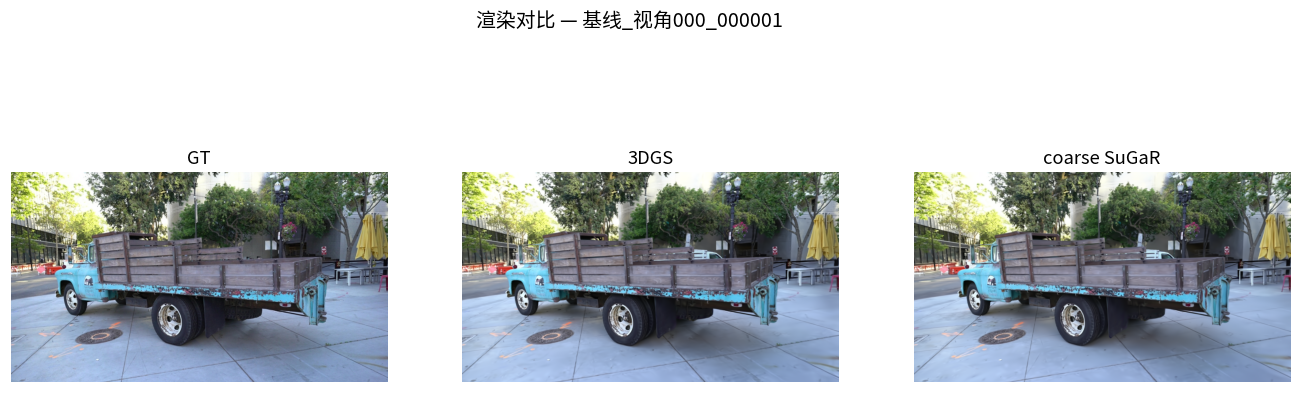
\includegraphics[width=\textwidth]{figures/渲染对比_基线_视角000_000001.png}
    \caption{测试视角渲染效果（视角~0）}
    \label{fig:baseline-render}
  \end{subfigure}
  \caption{基线 SuGaR Mesh 提取可视化（truck 场景）。
  (a) 整体网格；
  (b) 4{,}851 个连通分量以颜色区分，可见大量小碎片散布于主体之外；
  (c) 到参考点云的距离误差热图；
  (d) 从测试视角的渲染结果与真值对比。}
  \label{fig:baseline-vis}
\end{figure}

图~\ref{fig:heatmap-comparison} 以统一色标展示了基线与改动（$\tau{=}0.02$）
的几何误差热图对比。

\begin{figure}[htbp]
  \centering
  \begin{subfigure}[b]{0.48\textwidth}
    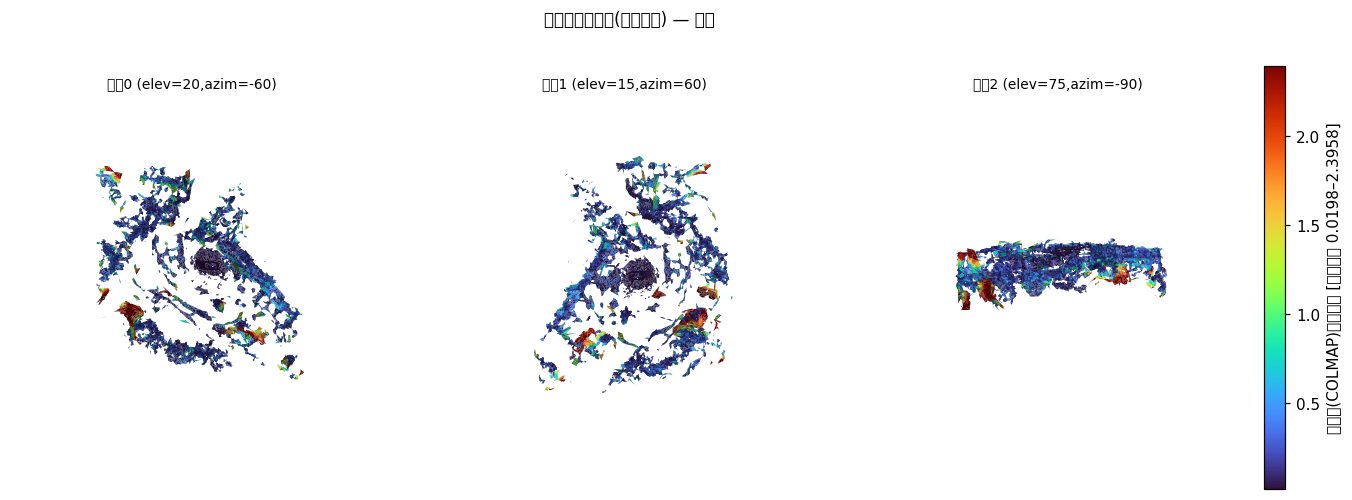
\includegraphics[width=\textwidth]{figures/误差热图_统一色标_基线.png}
    \caption{基线}
  \end{subfigure}
  \hfill
  \begin{subfigure}[b]{0.48\textwidth}
    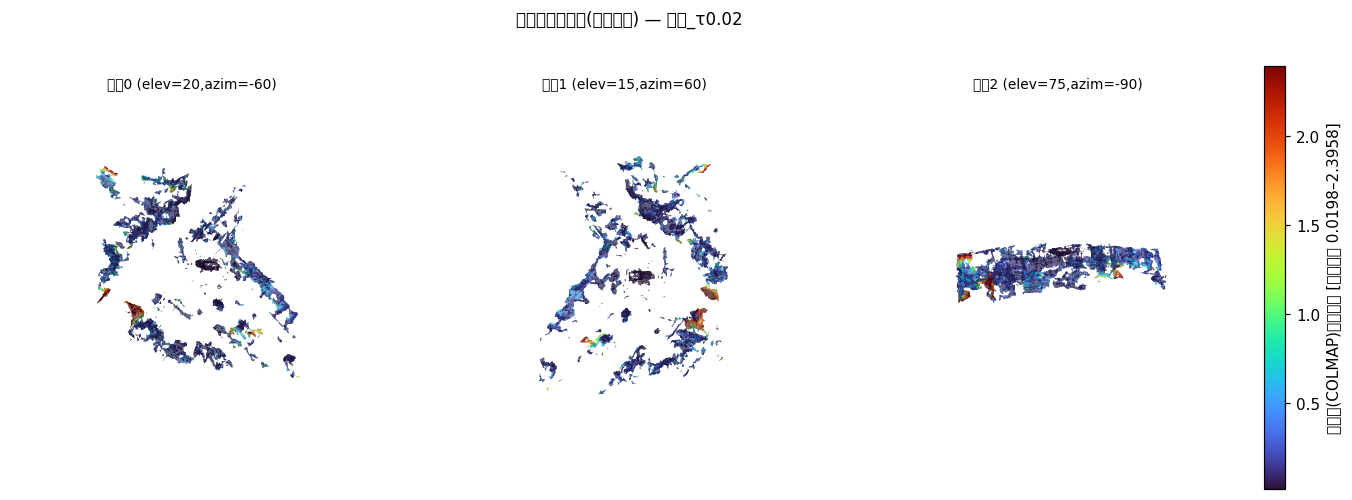
\includegraphics[width=\textwidth]{figures/误差热图_统一色标_改动_τ0.02.png}
    \caption{改动（$\tau{=}0.02$）}
  \end{subfigure}
  \caption{几何误差热图对比（统一色标，单位：场景坐标）。
  剔点后（右），远景区域的大面积高误差区显著减少，
  说明背景壳与漂浮几何被有效剔除；
  但前景主体边缘出现部分孔洞。}
  \label{fig:heatmap-comparison}
\end{figure}

\IfFileExists{figures/对比图_基线_vs_改动.pdf}{%
  \begin{figure}[htbp]
    \centering
    \includegraphics[width=\textwidth]{figures/对比图_基线_vs_改动.pdf}
    \caption{基线与改动（$\tau{=}0.02$）的综合可视化对比：
    网格整体视图、连通分量着色与渲染覆盖掩码。}
    \label{fig:overall-comparison}
  \end{figure}
}{}

% ---------- 基线观察 ----------
\subsubsection{基线观察}
\label{ssec:baseline-obs}

从表~\ref{tab:topo-cov-eff} 与图~\ref{fig:baseline-vis} 可以看出，
基线提取的网格包含~4{,}851 个连通分量，
但最大分量仅占全部面数的约~49.5\%，
说明近半数的三角面分布在数千个漂浮小块中。
这些漂浮几何导致~96{,}544 条边界边与~7{,}970 个孔洞，网格远非水密。
该现象与第~\ref{sssec:motivation}~节分析的单视角自洽但跨视角不一致的
表面采样点直接相关，为后续改动提供了明确的优化方向。

% =====================================================================
\subsection{超参敏感性与失败案例}
\label{ssec:sensitivity}

图~\ref{fig:tau-curve} 展示了剔除率随容差 $\tau$ 的变化趋势。
在固定 $k_{\min}{=}2$、$v_{\max}{=}1$、$M{=}30$ 的条件下，
剔除率随 $\tau$ 严格单调递减：
$\tau{=}0.005$ 时剔除 72.2\%，$\tau{=}0.2$ 时仅剔除 9.0\%。

\begin{figure}[htbp]
  \centering
  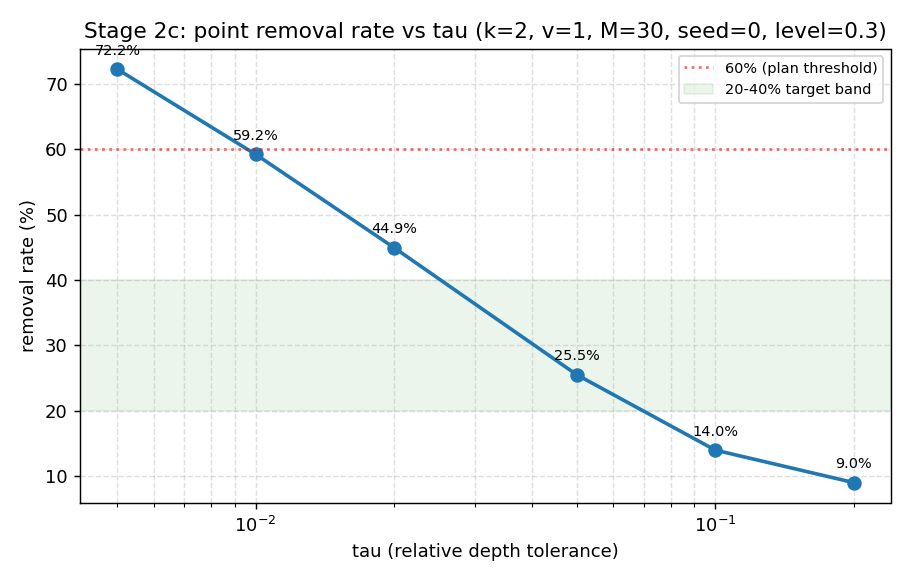
\includegraphics[width=0.65\textwidth]{figures/剔除率_随τ变化.png}
  \caption{剔除率随容差 $\tau$ 的变化（$k_{\min}{=}2$，$v_{\max}{=}1$，$M{=}30$）。
  $\tau$ 越小判据越严格，剔除的点越多。
  本实验选取 $\tau\in\{0.05,\,0.02,\,0.01\}$ 三点做完整提取与评测。}
  \label{fig:tau-curve}
\end{figure}

表~\ref{tab:geo-refA}--\ref{tab:topo-cov-eff} 揭示了 $\tau$ 驱动的一组权衡。
随着 $\tau$ 从 0.05 减小到 0.01：
\begin{itemize}[nosep]
  \item \textbf{改善方向}：连通分量（3{,}279 $\to$ 2{,}261）、
        孔洞（6{,}206 $\to$ 4{,}598）、边界边（68{,}205 $\to$ 44{,}848）
        持续下降；
        Chamfer 距离（参考 B）从 0.0455 降至 0.0361；
        F@1\%（参考 B）从 0.920 升至 0.963。
  \item \textbf{恶化方向}：网格覆盖率从 81.5\% 降至 63.3\%，
        前景漏洞率从 18.0\% 升至 36.3\%；
        Accuracy P90（参考 B）从 0.0239 升至 0.0287（变差 20\%），
        反映部分真实表面被误剔后参考点到最近网格面的距离增大。
\end{itemize}

\paragraph{失败案例：$\tau{=}0.01$。}
$\tau{=}0.01$ 剔除了 59.2\% 的表面点，覆盖率骤降至 63.3\%、
漏洞率飙升至 36.3\%。
虽然 Chamfer 距离仍在改善，但代价已远超收益：
真实表面因深度渲染的微小误差（离散化噪声、遮挡边界处的深度跳变）
被判为不一致而被剔除，形成大面积孔洞。
这一失败案例表明，$\tau$ 不应低于深度渲染本身的噪声水平。

\paragraph{推荐设置。}
$\tau{=}0.05$ 仅剔除 25.5\%，拓扑改善温和、覆盖损失可控（81.5\%）；
$\tau{=}0.02$ 剔除 44.9\%，几何收益更显著但覆盖降至 71.0\%。
二者的选择取决于下游任务对覆盖完整性与几何干净度的相对权重。

% =====================================================================
\subsection{分析}
\label{ssec:analysis}

\paragraph{改动带来了什么。}
多视角深度一致性剔点在所有 $\tau$ 设置下均显著降低了 Chamfer 距离
（参考 B：基线 0.0531 $\to$ $\tau{=}0.02$ 时 0.0390，降幅约 27\%）、
连通分量数（4{,}851 $\to$ 2{,}690，降幅 45\%）与孔洞数
（7{,}970 $\to$ 5{,}480，降幅 31\%）。
Completeness 均值大幅改善（参考 A：0.0495 $\to$ 0.0286，降幅 42\%），
表明漂浮于远离参考面的虚假网格面已被有效消除。
F-score 在所有阈值下均单调上升
（F@1\% 参考 B：0.888 $\to$ 0.949），
进一步证实剔点在保持召回率的同时大幅提升了精确率。
在 $\tau{=}0.05$ 时，最大分量面数占比从 49.5\% 升至 58.1\%，
意味着网格几何更集中于场景主体。

\paragraph{改动没有带来什么。}
渲染质量完全不变（PSNR 24.32\,dB、SSIM 0.848），
这是设计上的必然结果：改动仅作用于 Mesh 提取阶段，
Coarse SuGaR 模型未经重训练，其高斯分布不受影响。
此外，网格在任何 $\tau$ 下均未达到水密状态——
Poisson 重建本身产生开放边界，仅靠剔点无法弥补。

\paragraph{计算代价。}
过滤器本身的额外开销极小：渲染 30 个参考深度图约 0.3\,s，
投票判断约 0.2\,s，合计约 0.5\,s。
由于剔点后进入 Poisson 重建的点数减少，
总提取墙钟反而缩短——$\tau{=}0.02$ 时从 5.98\,min 降至 4.30\,min（快 28\%）。
峰值显存在 $\tau{=}0.02$ 下为 8{,}274\,MiB，低于基线的 10{,}098\,MiB。
因此，该改动在计算成本上几乎"免费"。

\paragraph{覆盖率下降是主要代价。}
网格覆盖率从基线的 92.9\% 降至 $\tau{=}0.02$ 时的 71.0\%，
前景漏洞率从 6.7\% 升至 28.6\%，
这是本改动的最大不足。
Accuracy P90（参考 B）从 0.0200 升至 0.0258（变差 29\%），
说明剔点误伤了部分真实表面，
使一些参考点失去了近邻网格面。

\paragraph{假设对照。}
实验结果逐条验证了三项预注册假设：

\begin{enumerate}[nosep,label=\textbf{H\arabic*}:]
  \item \textbf{几何改善}——
        连通分量数、Chamfer 距离、Completeness 均值三项均随剔点
        单调改善（\textbf{支持}）。
  \item \textbf{过剔损害覆盖}——
        $\tau$ 越小，覆盖率越低、漏洞率越高、Accuracy P90 越差；
        $\tau{=}0.01$ 构成典型的过度剔除案例（\textbf{支持}）。
  \item \textbf{渲染不变}——
        所有组别共享同一 Coarse 模型，PSNR / SSIM / LPIPS 恒等
        （\textbf{支持}）。
\end{enumerate}
